\documentclass[9pt]{beamer}
\usepackage[utf8]{inputenc}
\usepackage{enumitem}
\usepackage{graphicx}
\usepackage{array}
\usepackage{mdwlist}
\usepackage{floatrow}
\usepackage{hyperref}
\usepackage{listings}
\usepackage{alloy}
\usepackage{color}
\usepackage{nameref}

\graphicspath{ {img/} }

\makeatletter
\newcommand*{\currentname}{\@currentlabelname}
\makeatother

\newcounter{saveenumi}
\newcommand{\seti}{\setcounter{saveenumi}{\value{enumi}}}
\newcommand{\conti}{\setcounter{enumi}{\value{saveenumi}}}

\usetheme{Warsaw}

\AtBeginSection[]
{
  \begin{frame}
    \frametitle{Table of Contents}
		\setcounter{tocdepth}{2}
    \tableofcontents[currentsection]
  \end{frame}
}

\title{myTaxiService}
\subtitle{Requirements Analysis and Specifications Document}
\author{Jacopo Strada, Luca Riva}
\date{November 11, 2015}

\begin{document}

\maketitle

\section{Introduction}
\subsection{Purpose}
\begin{frame}{\currentname}
This document is meant to describe a software solution for the \emph{myTaxiService} problem. The document includes a description of the problem, functional and non-functional requirements and it is addressed to the IT department of the city administration.
\end{frame}

\subsection{Scope}
\begin{frame}{\currentname}
The \emph{myTaxiService} software focuses on helping the clients benefit from the service and ensures a fair management of taxi queues.
\end{frame}

\subsubsection{Goals}
\begin{frame}{\currentname{} I}

\begin{enumerate}[label=\bfseries G\arabic*:]
\item Allow clients to register an account in the system
\item Allow taxi drivers to register an account in the system
\item Allow clients to log in the mobile application or in the website
\item Allow taxi drivers to log in the mobile application
\item Allow clients to request a taxi
\item Inform the passenger about the code of the incoming taxi
\item Inform the passenger about the waiting time
\item Inform the passenger about a possible call rejection
\seti
\end{enumerate}
\end{frame}

\begin{frame}{\currentname{} II}
\begin{enumerate}[label=\bfseries G\arabic*:]
\conti
\item Retrieve the position of each taxi from their mobile application using GPS
\item Allow taxi drivers to set their state as \emph{available} or \emph{unavailable}
\item Notify the taxi drivers about a client's request
\item Allow taxi drivers to accept or decline a certain client's request
\item Guarantee a fair management of taxi queues
\item Allow a user to reserve a taxi by specifying the origin and the destination of the ride at least two hours before
\item Allow a driver to accept a client reservation
\item Confirm the reservation to the user
\item Supply APIs for further implementation of additional services in the future
\end{enumerate}
\end{frame}

\section{Overall Description}
\subsection{Product perspective}
\begin{frame}{\currentname}
The software will consist in three different user interfaces: two different apps for the clients and the taxi drivers and one web application. 

In order to make this working there will be a web server containing the application logic and a DBMS that stores all the data (such as users' credentials, taxi's positions, taxi's availability \ldots).
Mobile applications, web application and the server communicate through the Internet.

The system will also provide programmatic interfaces for other new services. At the moment the city has not any similar system, so the application will be completely independent.
\end{frame}

\subsection{User characteristics}
\begin{frame}{\currentname}
This application is conceived for every taxi driver in the city area and for adult clients (18+) with a compatible device which satisfies the specification listed in the previous section. There are no specific levels of education or expertise needed apart from a decent knowledge of English language.
\end{frame}

\subsection{Domain properties}
\begin{frame}{\currentname}
\begin{enumerate}[label=\bfseries D\arabic*:]
\item If a client requests a ride they will wait the taxi's arrival
\item If a client makes a reservation for a certain time they will be punctual waiting for the ride
\item If a driver accepts a reservation or a request they will actually try to reach the client location
\end{enumerate}
\end{frame}

\subsection{Assumptions}
\begin{frame}{\currentname{} I}
\begin{enumerate}[label=\bfseries A\arabic*:]
\item Possibility to gain access to the taxi driver's licences database of the city
\item A client is able to make only one taxi request at once
\item A client is not able to make two overlapped reservations
\item If a request is rejected by all the taxi drivers in the queue the request will be discarded: it will not iterate the queue for a second time.
\item As soon as the request is discarded the client will be notified and able to make a new call
\item The system will not give the client any information regarding the cost of the ride
\item If a client calls a taxi and the request is accepted the client will not be able to modify or erase the request.
\seti
\end{enumerate}

\end{frame}
\begin{frame}{\currentname{} II}

In order to assure an efficient service it is necessary a slight modification to the customer request:

\begin{enumerate}[label=\bfseries A\arabic*:]
\conti
\item When a customer reserves a taxi the system allocates the request to all registered driver
\item If a driver accepts the request the system confirms the reservation to the user
\item If no driver confirms the reservation in at most an hour since the request the system deletes the reservation and notifies the client
\item A taxi reservation's origin must be located inside one of the zones of the city
\item A client is able to cancel a reservation at least ten minutes before the ride.
\item The system notifies the driver about the ride they accepted ten minutes before the hour of the appointment with the client
\end{enumerate}

Assumptions A8, A9, A10, A13 were made in order to avoid the risk of having an empty queue or no driver who would accept the reservation only ten minutes before the fixed hour of the ride.
\end{frame}

\subsection{Apportioning of requirements}
\begin{frame}{\currentname{} I}
\begin{description}
\item[Reporting:] A client may report the lack of service of a driver so that the city's government would be able to take action against the said driver. At the same time a driver may be able to report a client who misses fixed appointments, thus after few reclaims the client's account could be suspended or deactivated. 
\item[Payments:] It would be interesting to give the client the possibility to pay the reservation service directly through the system, which could also provide an estimated price for the ride given the origin and the destination.
\end{description}
\end{frame}
\begin{frame}{\currentname{} II}
\begin{description}
\item[Taxi sharing:] An user may be ready to share a taxi, so the application could mark their requests in order to allow other clients to participate in the ride if they have a similar starting point and a similar destination. Obviously the advantage wold be the possibility to split the cost of the ride, which should be calculated by the system. The system should also compute the route for the taxi driver.
\end{description}
\end{frame}

\section{Specific requirements}

\subsection{User Interfaces}
\subsubsection{Clients' User Interfaces}
\begin{frame}{\currentname{} - Taxi Call}
\begin{columns}[c]
  \begin{column}{.5\textwidth}
		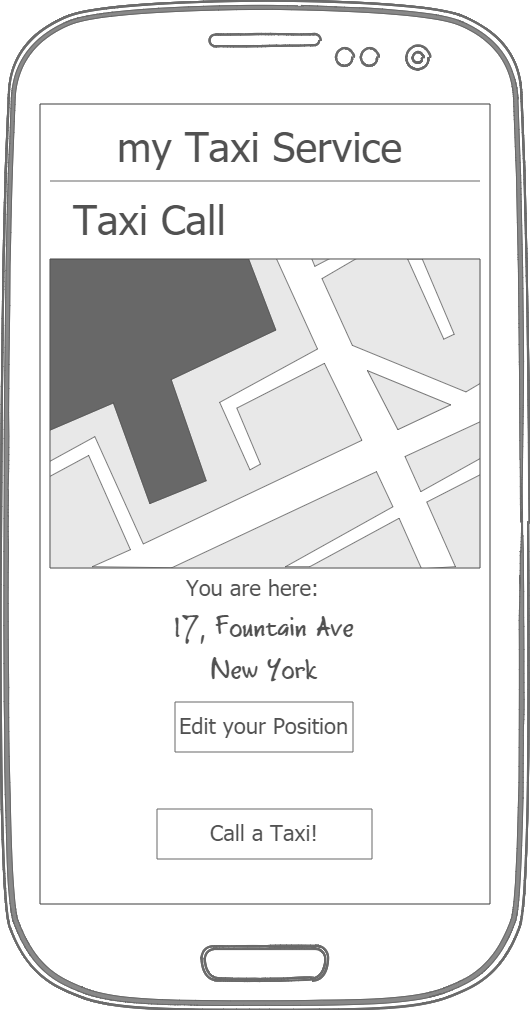
\includegraphics[height=.8\textheight]{Mockup-ClientsTaxiCall}
		\centering
  \end{column}
  \begin{column}{.5\textwidth}
    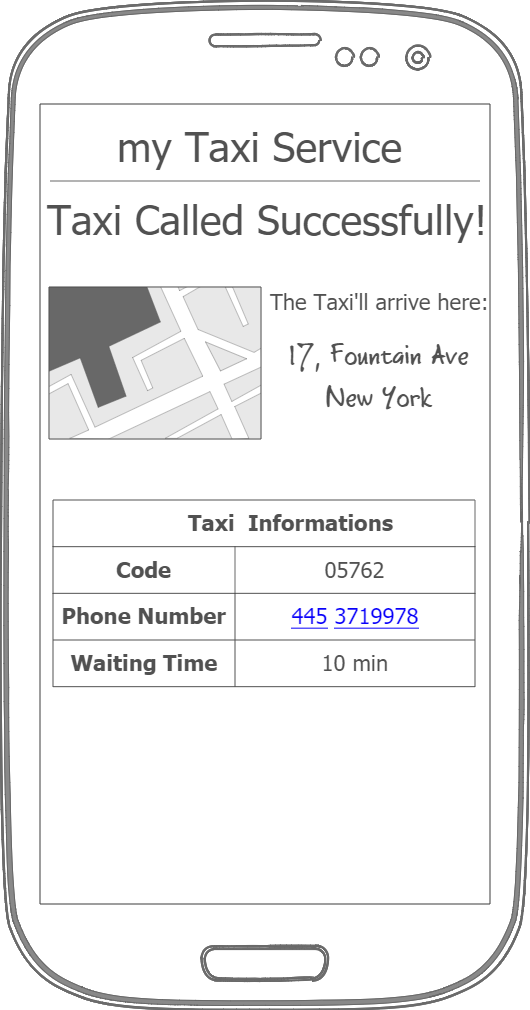
\includegraphics[height=.8\textheight]{Mockup-ClientsTaxiCallConfirmation}
		\centering
  \end{column}
\end{columns}
\end{frame}

\subsubsection{Taxi Drivers' User Interfaces}
\begin{frame}{\currentname{} - New Requests}
\begin{columns}[c]
  \begin{column}{.5\textwidth}
		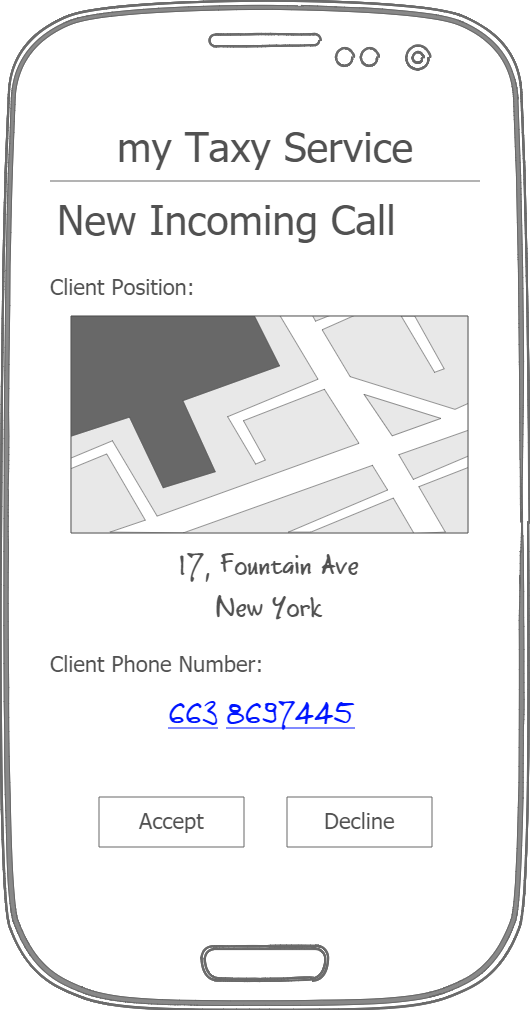
\includegraphics[height=.8\textheight]{Mockup-TaxiDriversNewIncomingCall}
		\centering
  \end{column}
  \begin{column}{.5\textwidth}
    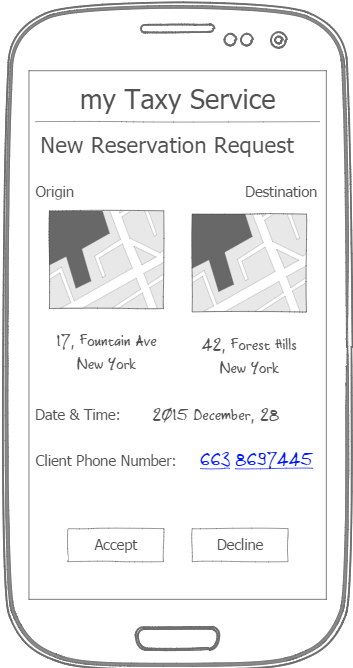
\includegraphics[height=.8\textheight]{Mockup-TaxiDriversReservationRequest}
		\centering
  \end{column}
\end{columns}
\end{frame}

\subsection{The World and The Machine}
\begin{frame}{\currentname}
The model by M. Jackson \& P. Zave is able to clearly schematize where the entities involved in the project are ideally located and which are the means of interaction between the world and the system at a first glance.

\begin{figure}[H]
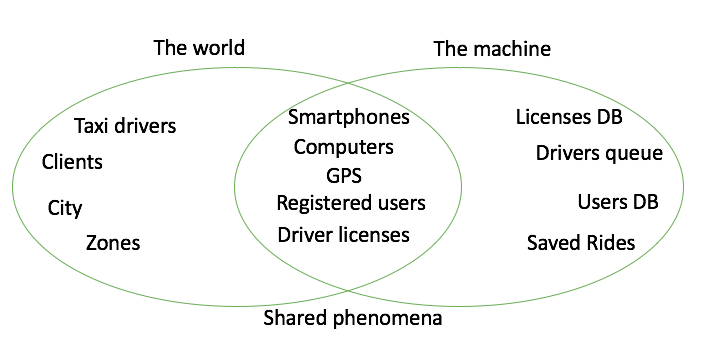
\includegraphics[height=0.5\textheight]{WorldAndMachine}
\centering
\end{figure}
\end{frame}

\subsection{Models}
\subsubsection{Use Case Models}
\begin{frame}{Clients UML use case diagrams}
\begin{figure}[H]
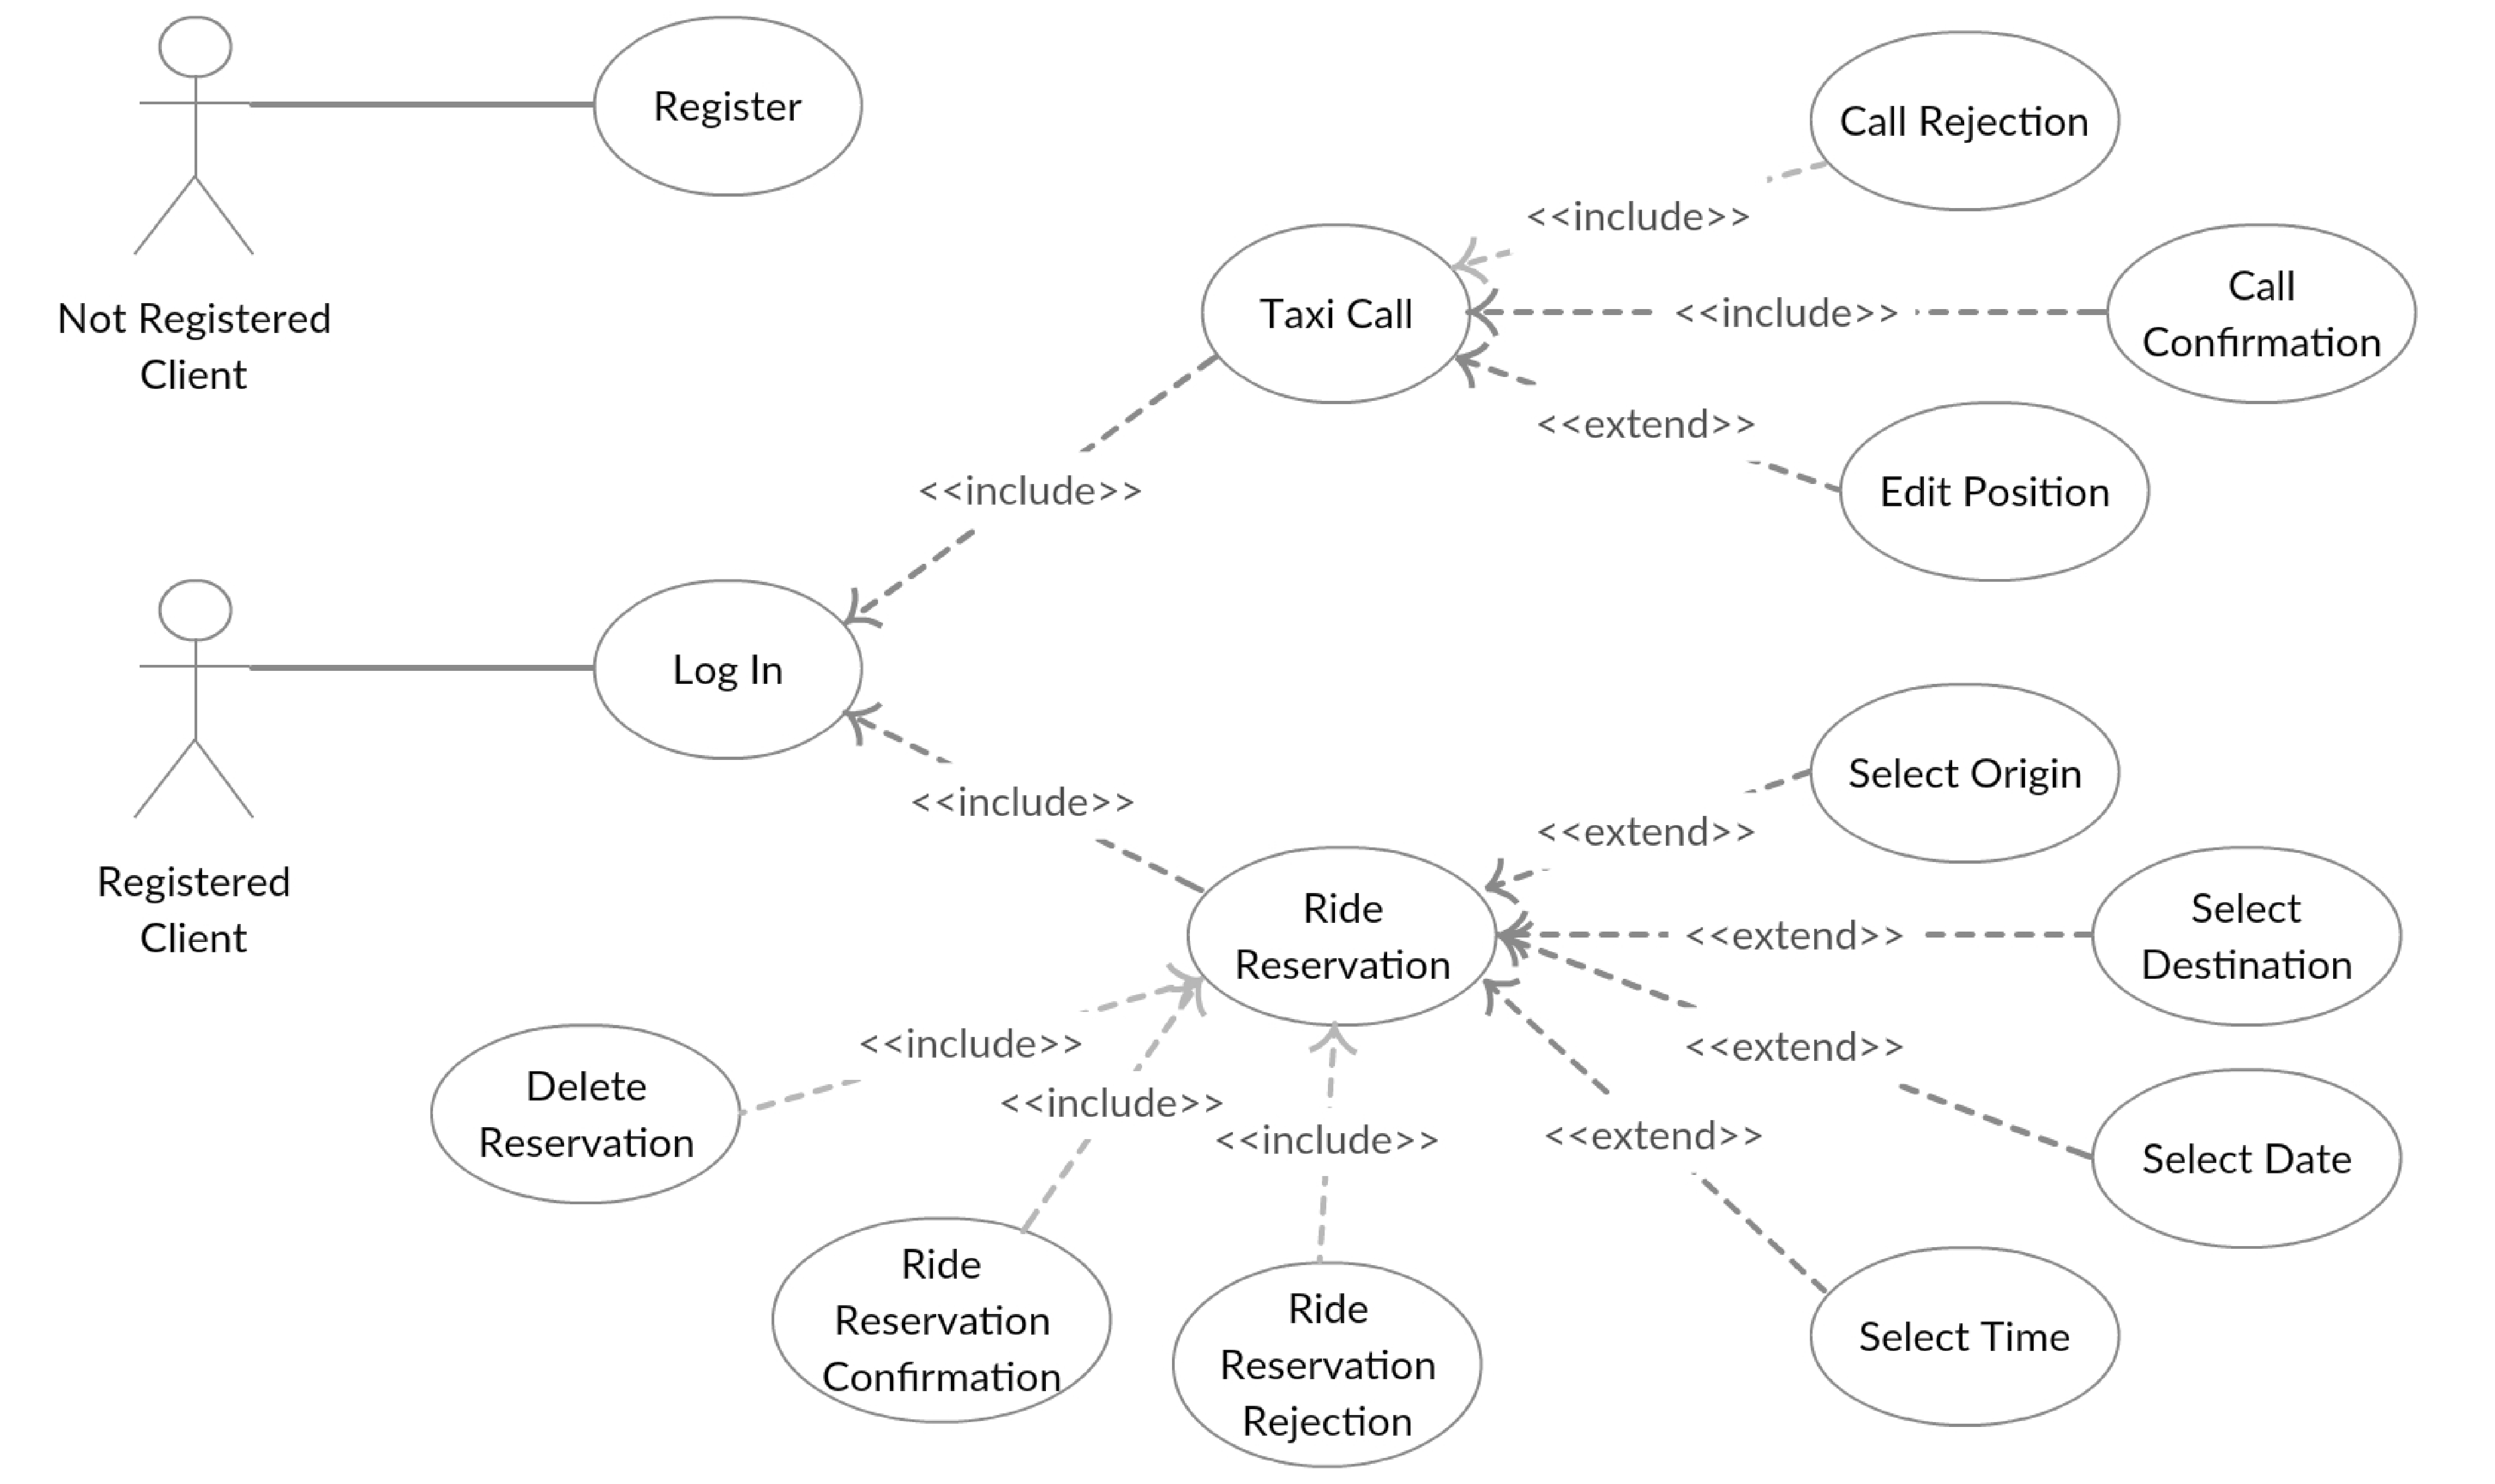
\includegraphics[height=0.8\textheight]{UseCase-Client}
\centering
\label{fig:usecaseclient}
\end{figure}
\end{frame}

\begin{frame}{Taxi Drivers UML use case diagrams}
\begin{figure}[H]
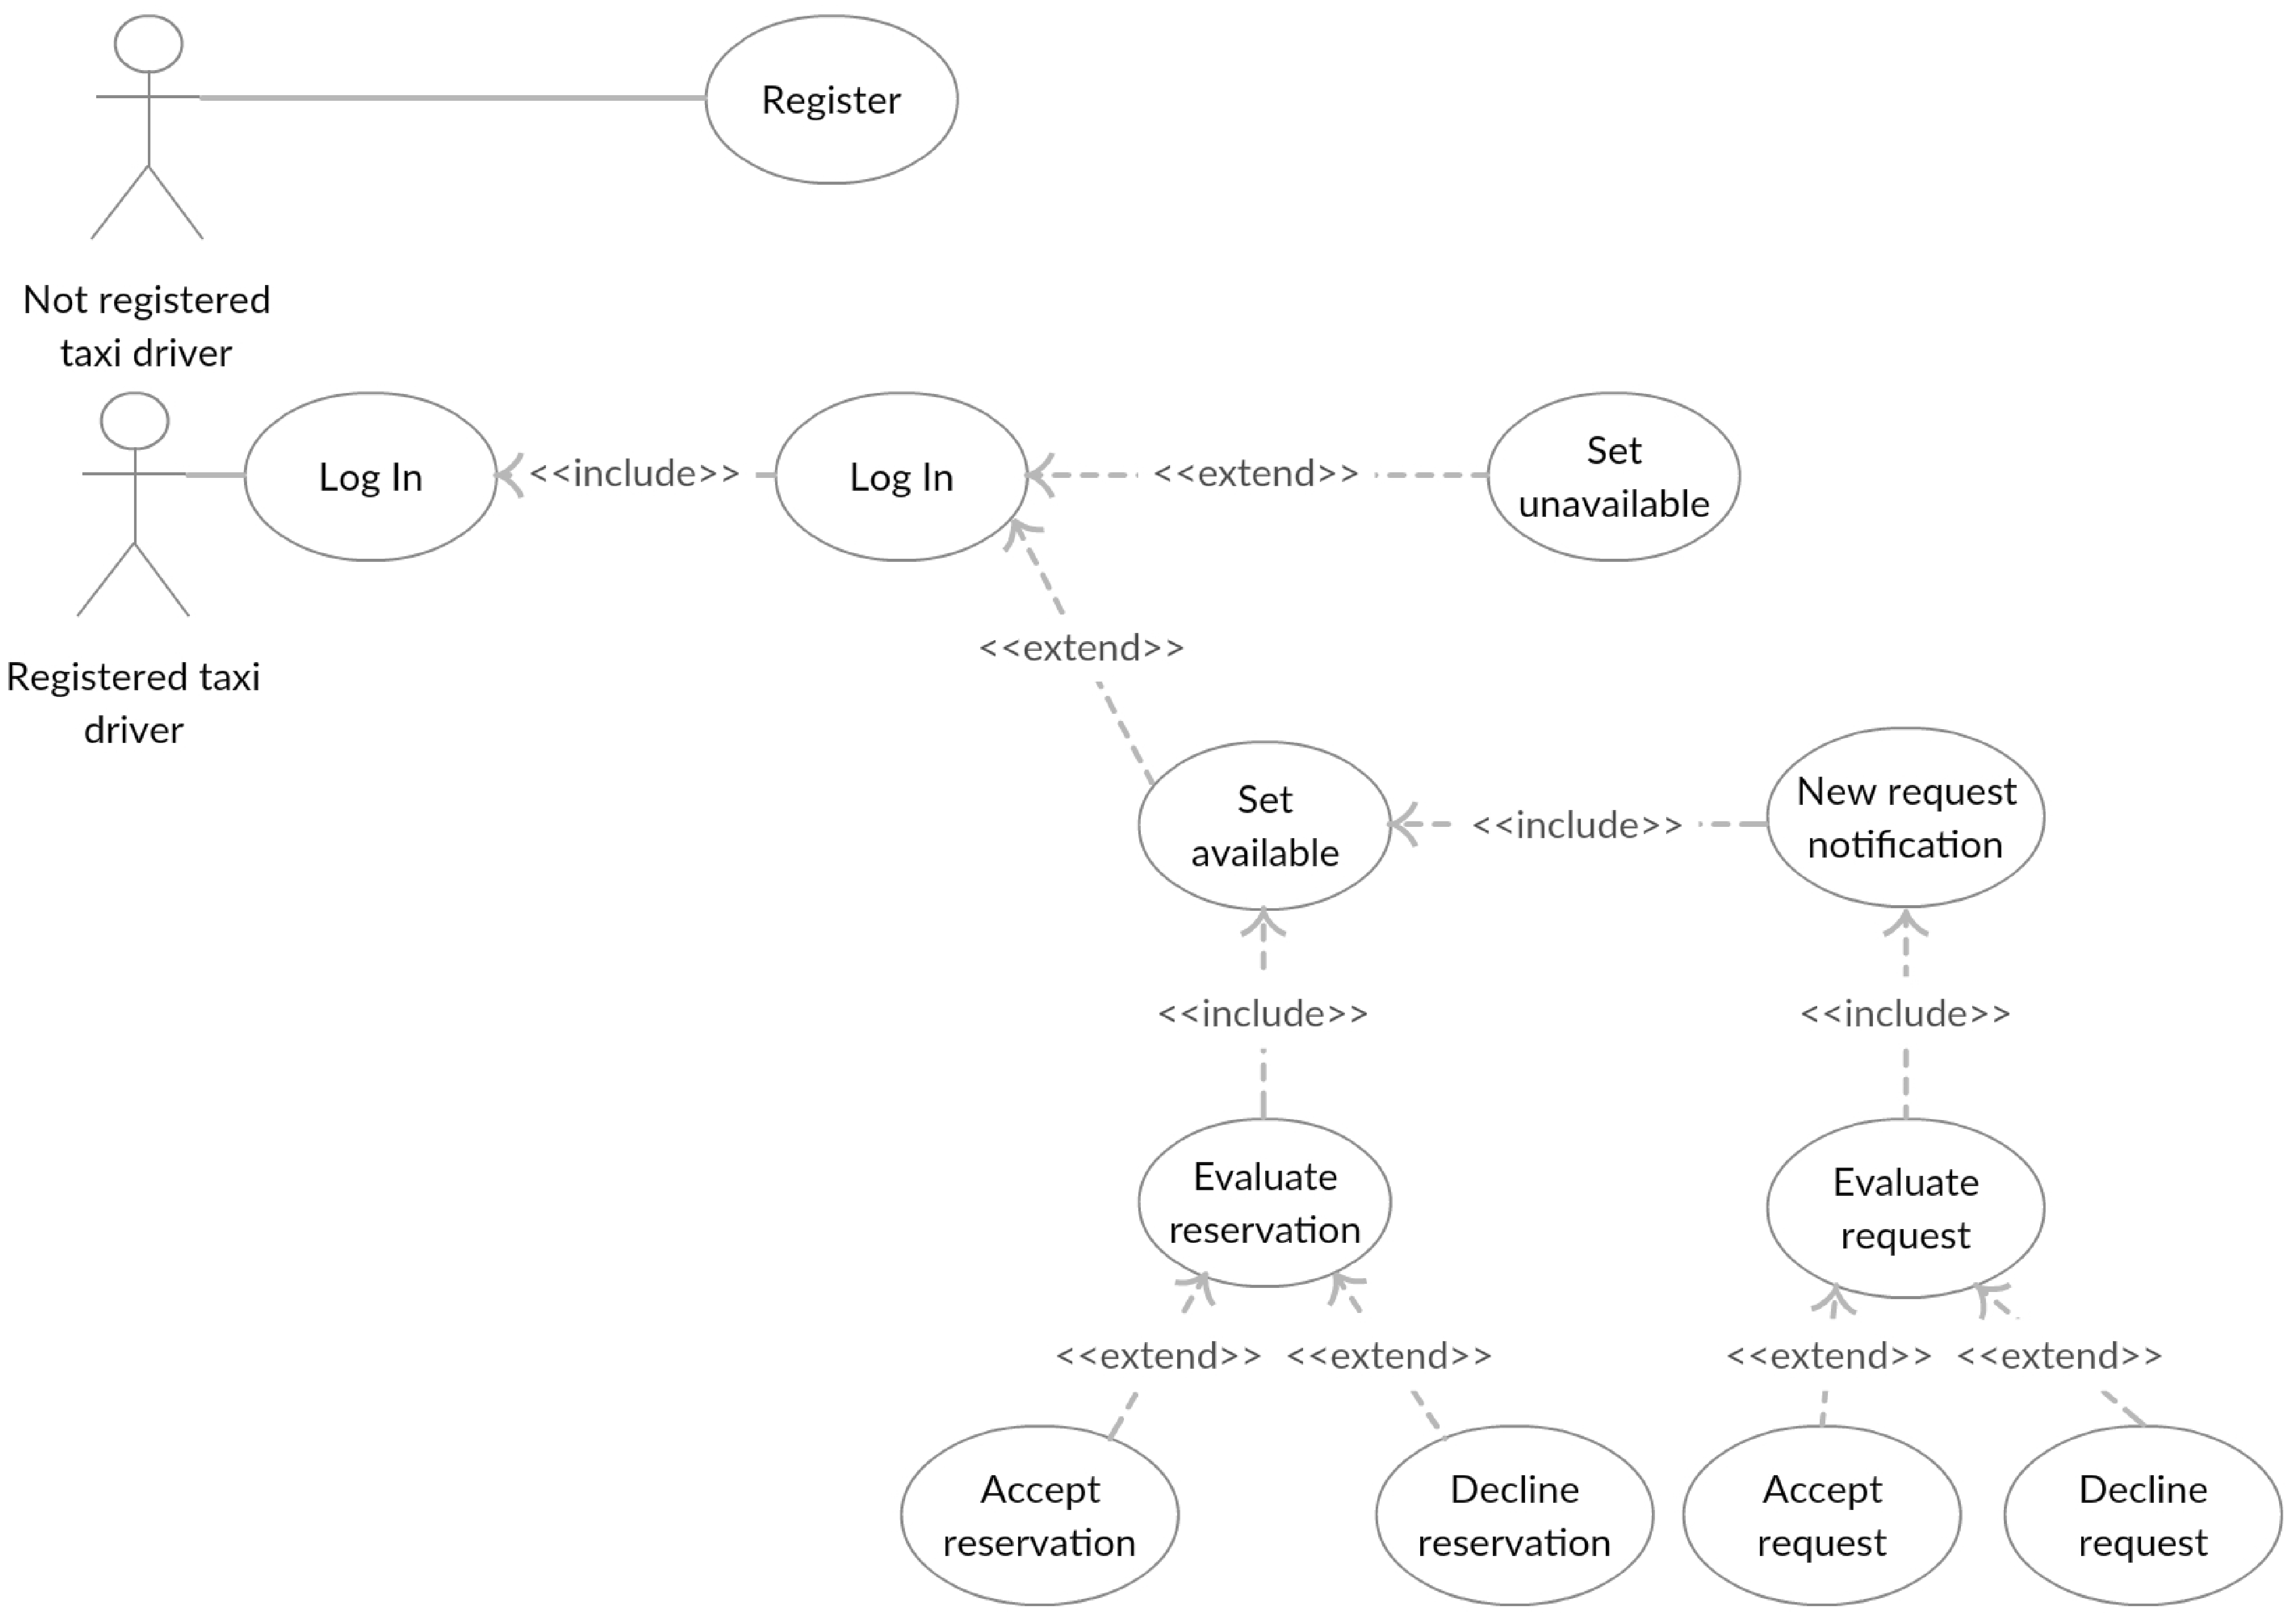
\includegraphics[height=0.8\textheight]{UseCase-TaxiDriver}
\centering
\label{fig:usecasetaxidriver}
\end{figure}
\end{frame}

\subsubsection{Sequence Diagrams}
\begin{frame}{Taxi call UML sequence diagram}
\begin{figure}[H]
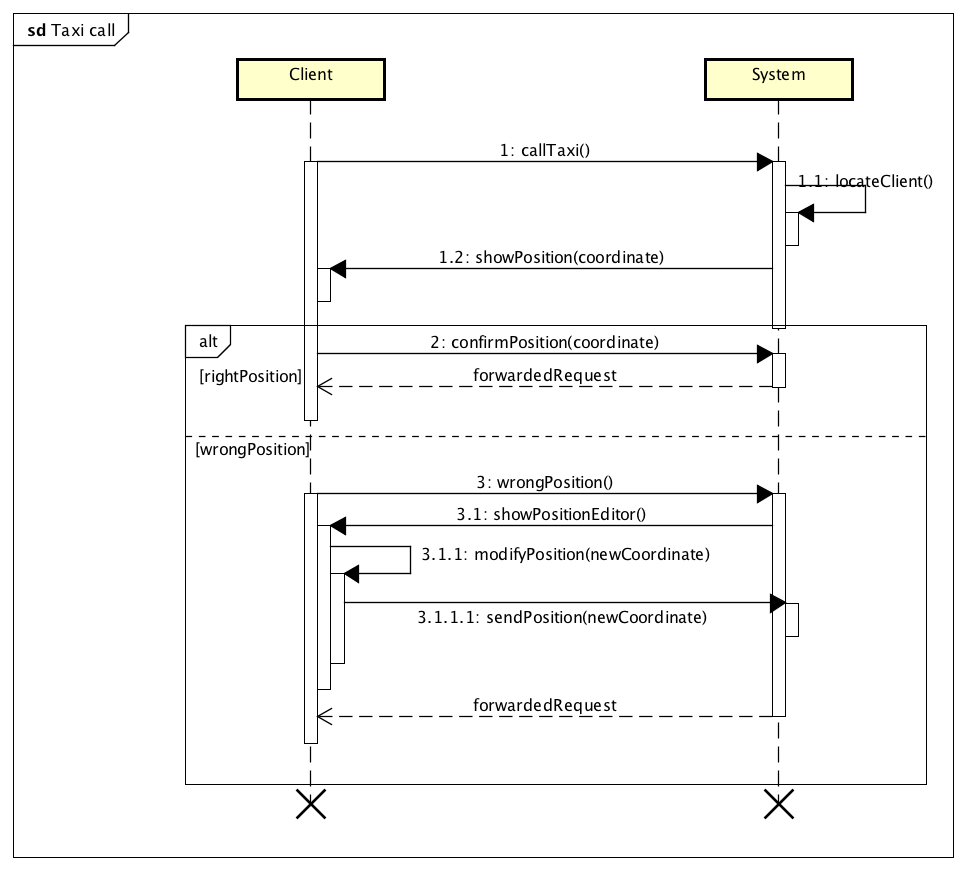
\includegraphics[height=0.8\textheight]{Sequence-Client-TaxiCall}
\centering
\label{fig:sequenceclienttaxicall}
\end{figure}
\end{frame}

\begin{frame}{Taxi reservation UML sequence diagram}
\begin{figure}[H]
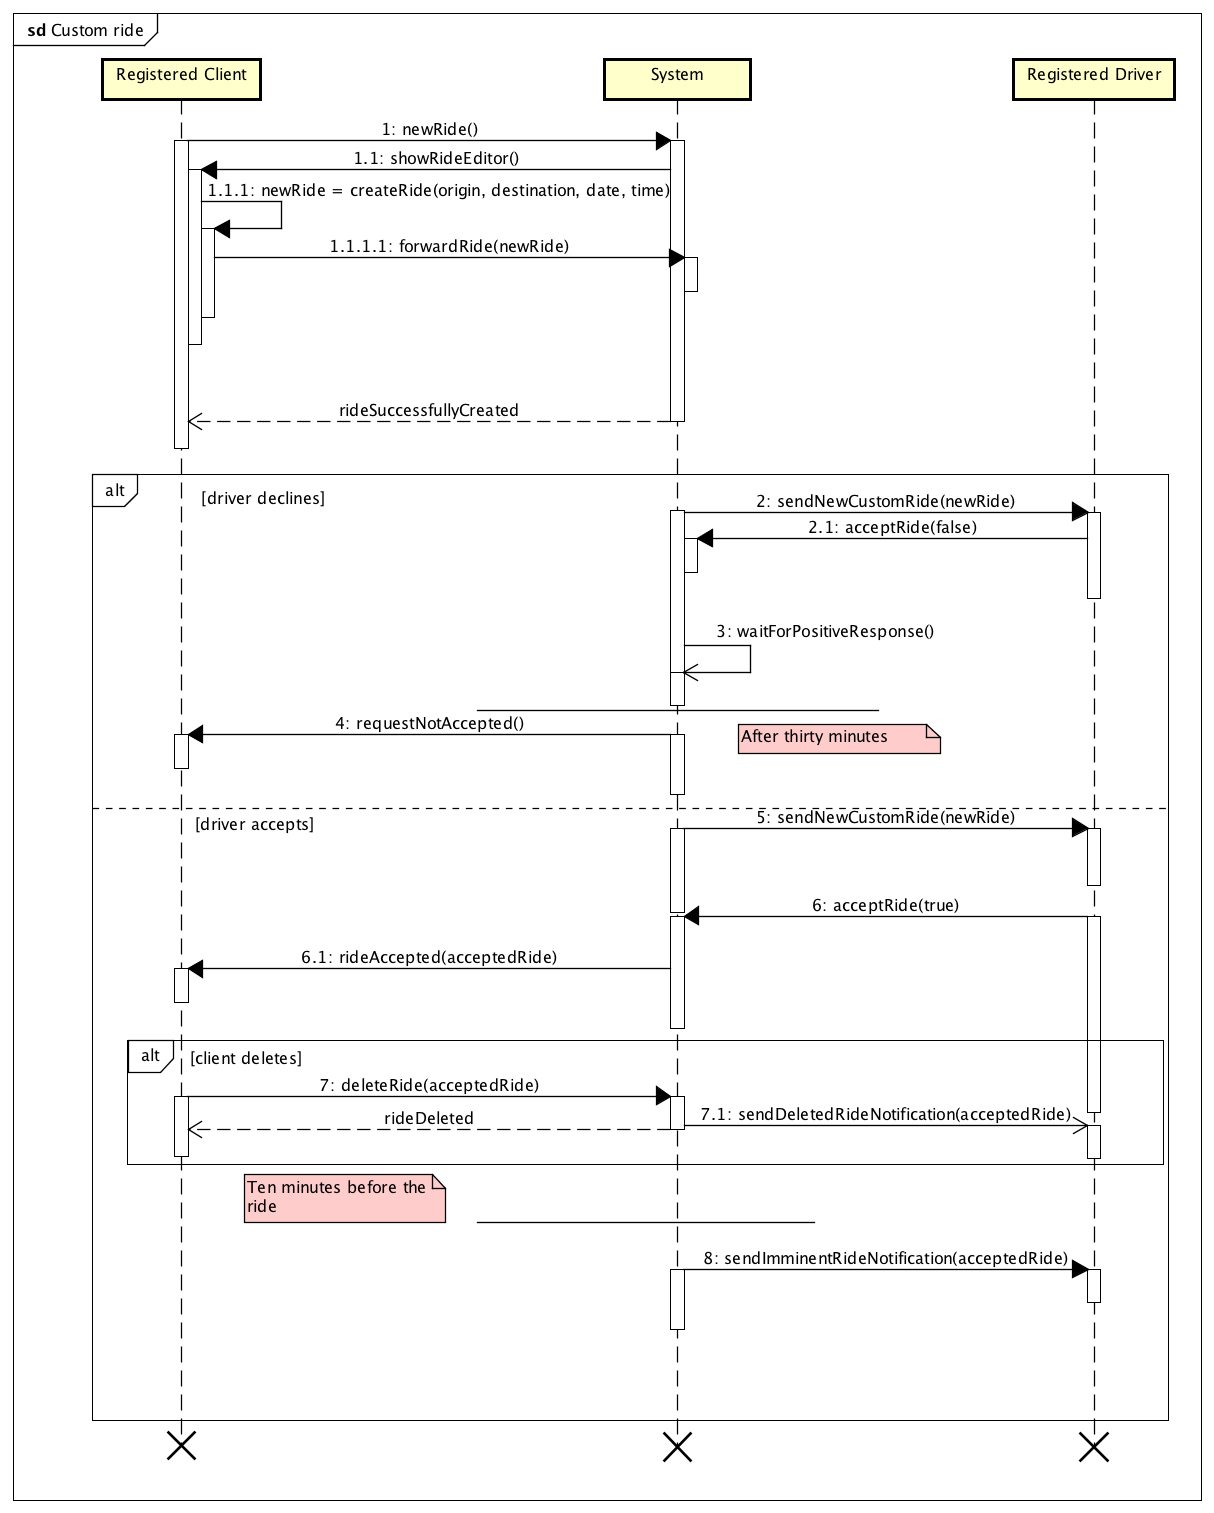
\includegraphics[height=0.8\textheight]{Sequence-Client-RideReservation}
\centering
\label{fig:sequenceclientridereservation}
\end{figure}
\end{frame}

\subsubsection{BPMN Diagrams}
\begin{frame}{BPMN taxi call}
\begin{figure}[H]
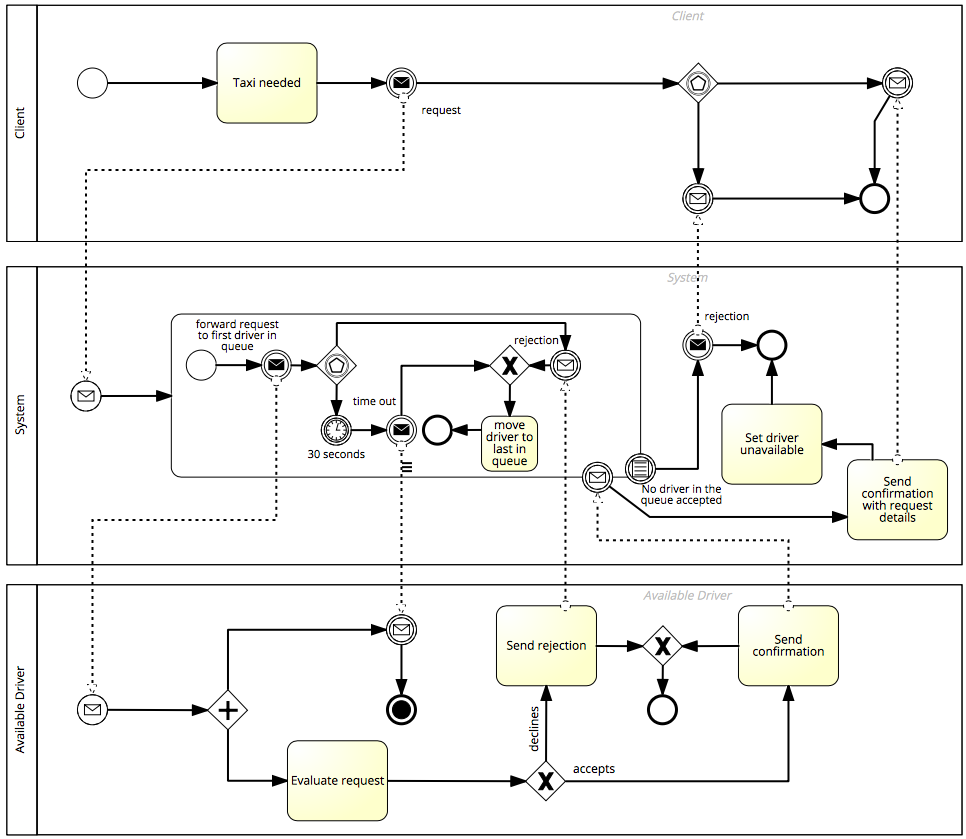
\includegraphics[height=0.8\textheight]{BPMN-rideRequest}
\centering
\label{fig:bpmndiagramrequest}
\end{figure}
\end{frame}

\begin{frame}{BPMN ride reservation}
\begin{figure}[H]
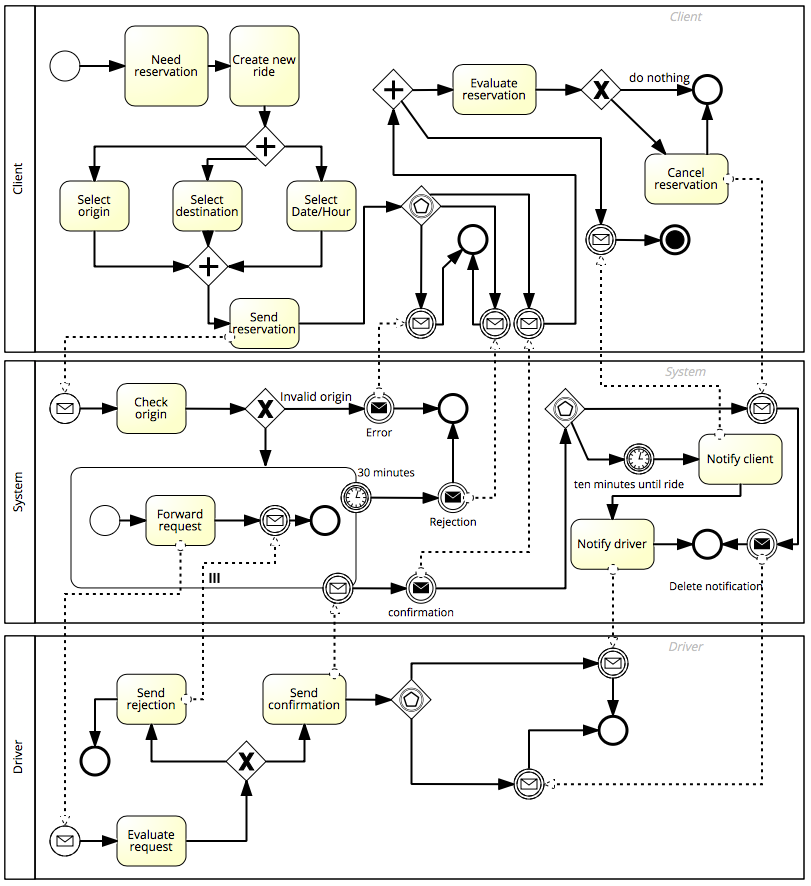
\includegraphics[height=0.8\textheight]{BPMN-rideReservation}
\centering
\label{fig:bpmndiagramreservation}
\end{figure}
\end{frame}


\section{Appendixes}
\subsection{Alloy}
\subsubsection{Signatures}

\begin{frame}[allowframebreaks]{\currentname}
\lstinputlisting[language=alloy]{alloy/signatures.als}
\end{frame}

\subsubsection{Facts}

\begin{frame}[allowframebreaks]{\currentname}
\lstinputlisting[language=alloy]{alloy/facts.als}
\end{frame}

\subsubsection{Worlds}

\begin{frame}{\currentname{} I}
\begin{figure}[H]
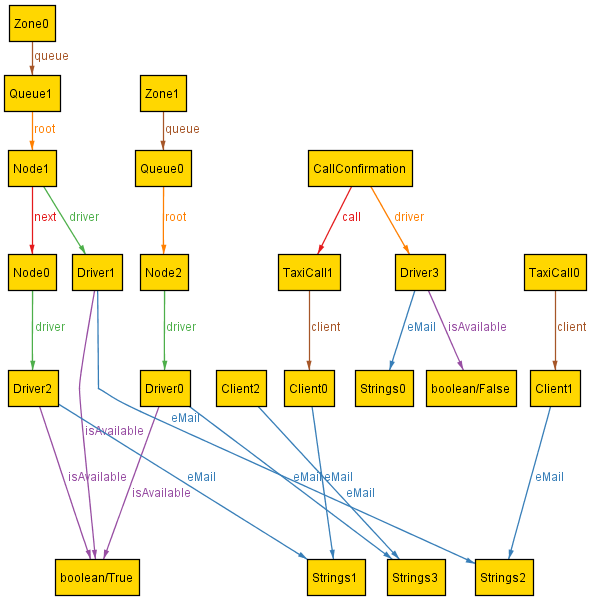
\includegraphics[height=0.8\textheight]{Alloy-Generic}
\centering
\label{fig:alloyworldgeneric}
\end{figure}
\end{frame}

\begin{frame}{\currentname{} II}
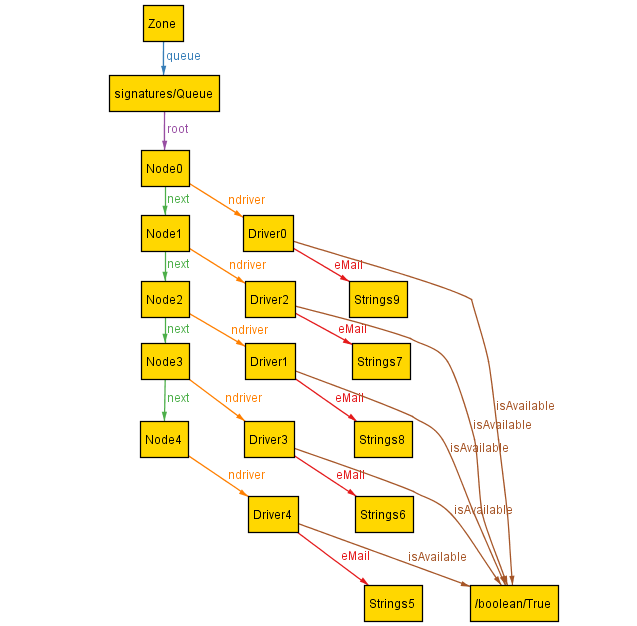
\includegraphics[height=0.8\textheight]{Alloy-AllAvailable}
\centering
\label{fig:alloyworldallavailable}
\end{frame}

\begin{frame}{\currentname{} III}
\begin{figure}[H]
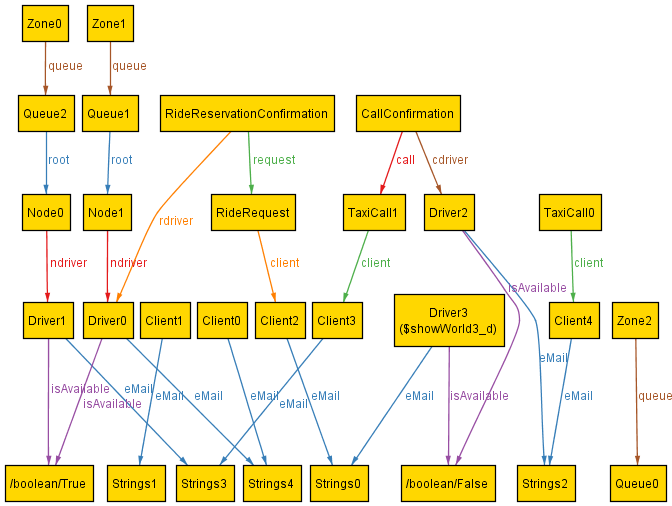
\includegraphics[height=0.8\textheight]{Alloy-FreeDriver}
\centering
\label{fig:alloyworldfreedriver}
\end{figure}
\end{frame}

\begin{frame}{\currentname{} IV}
\begin{figure}[H]
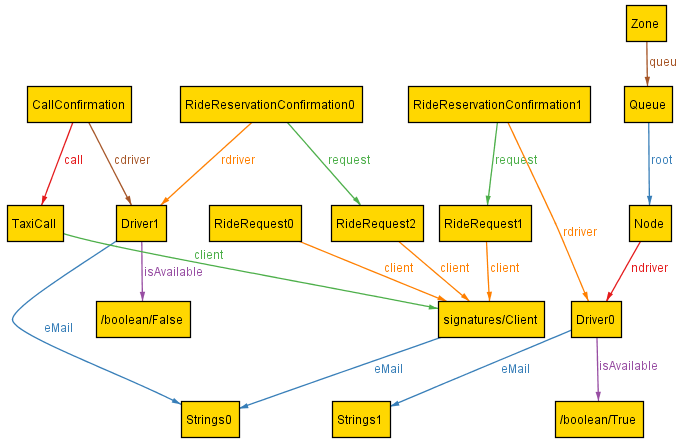
\includegraphics[height=0.8\textheight]{Alloy-RideReservation}
\centering
\label{fig:alloyworldridereservation}
\end{figure}
\end{frame}

\end{document}